\section{Processi interni}

Le informazioni qui riportate derivano da osservazione diretta del mio ambiente di lavoro e da confronti brevi con il tutor interno; 
durante i due mesi di stage ho svolto il progetto in larga parte in autonomia, perciò la mia percezione dei processi si basa prevalentemente su quanto mi è stato illustrato dal tutor aziendale 
e su alcune conversazioni avute con i membri del \emph{team}, e non pretende di essere esaustiva.

\medskip
\noindent\textbf{Processo di sviluppo}

Il processo di sviluppo si articola in fasi distinte ma integrate: individuazione e definizione del problema, 
scomposizione in attività eseguibili, implementazione, verifica e rilascio. 
Per la gestione del codice e del \emph{versioning} si utilizzano strumenti dedicati (controllo di versione distribuito, repository remoti) e, 
parallelamente, si impiegano sistemi per tracciare le attività e le priorità. Dalle conversazioni tra i membri del \emph{team} ho rilevato l’esistenza di una fase iniziale di 
analisi in cui il problema viene chiarito e suddiviso in \emph{task} di dimensione tale da poter essere assegnata a un singolo sviluppatore; questa scomposizione agevola la 
responsabilizzazione dei singoli e il monitoraggio dei progressi.

Lo strumento visivamente riconoscibile per la creazione, 
l’assegnazione e il monitoraggio delle \emph{tasks} è \emph{Jira}, che funge da punto di riferimento per lo stato dei lavori, le descrizioni delle attività e i commenti di avanzamento. 
Durante la fase di sviluppo giornaliera sono previste brevi \emph{stand-up meetings} (riunioni di sincronizzazione) con l’obiettivo di condividere quanto svolto nella giornata precedente, 
segnalare impedimenti e pianificare le attività immediate; queste riunioni favoriscono l’allineamento del \emph{team} e la rapida emersione di blocchi tecnici.

Al completamento di ogni \emph{task} è prevista una fase di verifica da parte di un altro membro del \emph{team} (code review): 
tale pratica viene svolta sia per assicurare qualità e conformità agli standard interni sia per favorire la diffusione delle conoscenze. 
Quando possibile, il rilascio del codice avviene seguendo procedure automatizzate che includono build e test automatici; ove presenti, 
pipeline di integrazione continua vengono attivate prima del merge verso i rami principali, riducendo il rischio di regressioni.

\begin{figure}[htbp]
    \centering
    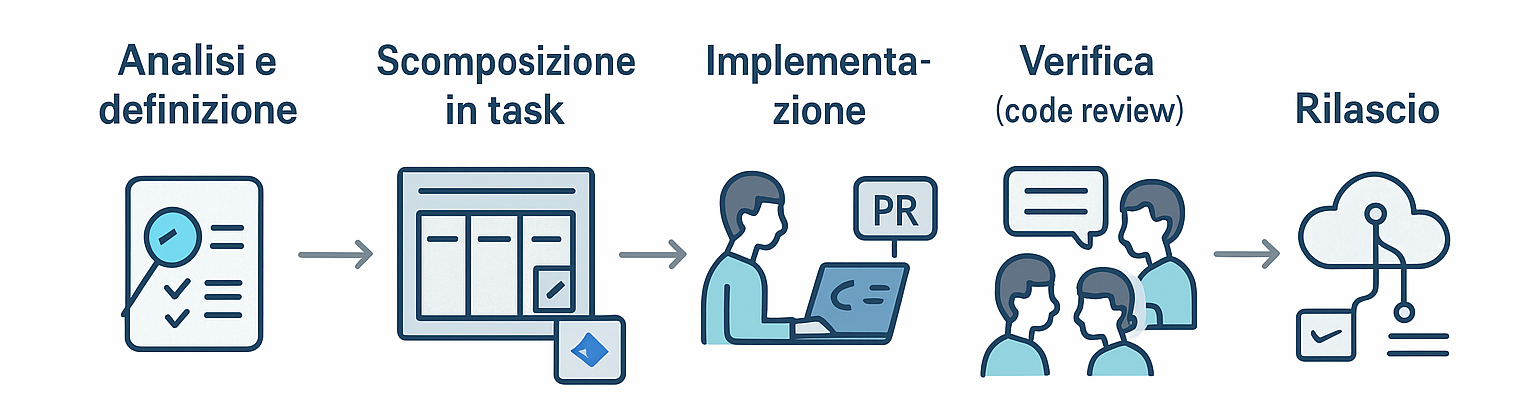
\includegraphics[width=0.9\textwidth]{images/azienda/processo_sviluppo}
    \caption{Flusso del processo di sviluppo adottato, dalle fasi di analisi al rilascio, con tracciamento in Jira e procedure automatizzate di integrazione continua.}
    \label{fig:processo_sviluppo}
\end{figure}

%Analisi → Scomposizione in task → Implementazione → Code review → Test → Rilascio

\medskip
\noindent\textbf{Processo di organizzazione}

L’organizzazione della comunicazione è stratificata in base al livello di formalità e alla finalità: 
comunicazioni rapide e operative avvengono su \emph{Slack}, che viene utilizzato per la pianificazione quotidiana delle presenze, richieste logistiche e notifiche veloci; 
per questioni tecniche più specifiche e per lo scambio su singole \emph{tasks} si sfruttano i \emph{branches} e i commenti collegati alle issue in \emph{Jira}, 
dove rimane tracciata la cronologia delle decisioni e delle discussioni tecniche. Le comunicazioni formali, amministrative o di carattere aziendale più strutturato vengono invece inviate tramite \emph{email}.

La documentazione di progetto è mantenuta in repository condivisi o in spazi dedicati (wiki, documenti di progetto): 
questo facilita il reperimento di informazioni, la consultazione delle linee guida e la storage delle specifiche. 
Ho notato che, nonostante esista una struttura di comunicazione definita, la pratica quotidiana lascia spazio a scambi informali che spesso risolvono rapidamente piccoli 
problemi ma che possono anche richiedere successiva formalizzazione quando le decisioni impattano sul piano di rilascio.

Non sono stato coinvolto nelle attività di manutenzione continuativa del sistema, né ho avuto discussioni approfondite con il tutor o con i membri del \emph{team} su procedure 
operative relative al supporto post-rilascio; pertanto non posso fornire dettagli completi su quel processo.


\begin{figure}[htbp]
    \centering
    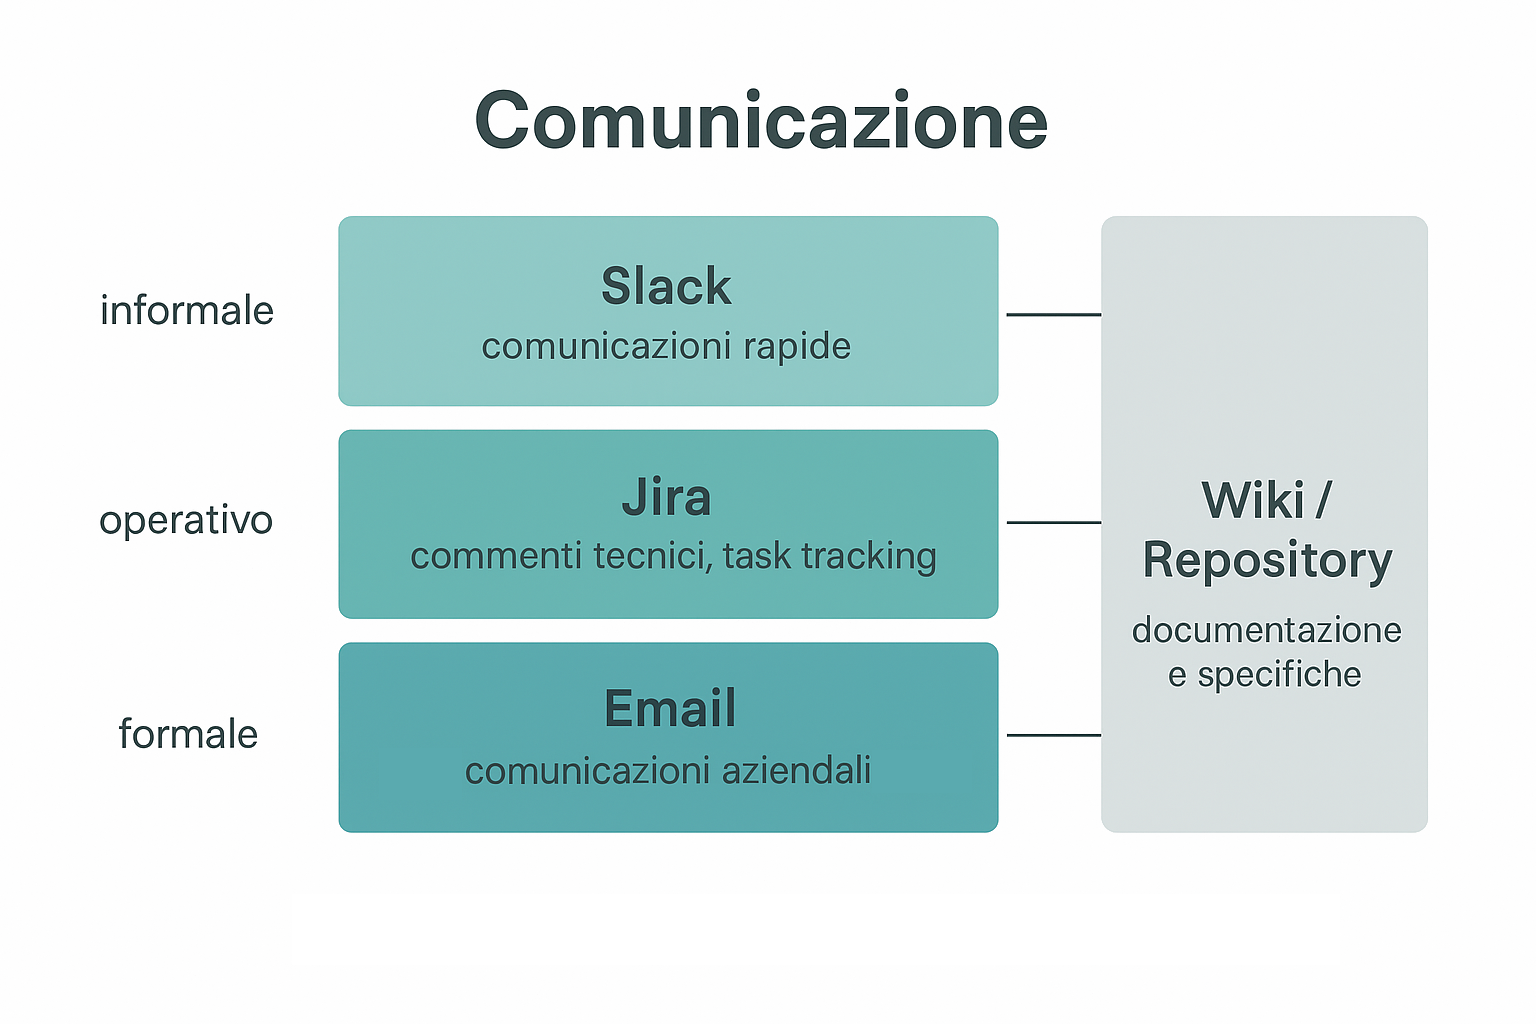
\includegraphics[width=0.9\textwidth]{images/azienda/comunicazione}
    \caption{Struttura dei canali di comunicazione interni e grado di formalità associato.}
    \label{fig:comunicazione}
\end{figure}

%Livello 1 (informale): Slack → comunicazioni rapide, Livello 2 (operativo): Jira → commenti tecnici, task tracking, Livello 3 (formale): Email → comunicazioni aziendali, amministrative, Livello trasversale: Wiki / Repository → documentazione e specifiche


\medskip
\noindent\textbf{Osservazioni riassuntive e suggerimenti}

Dall’esperienza osservativa emergono alcuni punti di forza e margini di miglioramento: la presenza di pratiche consolidate (uso di \emph{Jira}, \emph{stand-up meetings}, code review) 
favorisce trasparenza e tracciabilità, mentre l’adozione più ampia di procedure formali per la documentazione delle decisioni tecniche potrebbe ridurre la dipendenza dalle comunicazioni informali. 
Sarebbe utile, a mio avviso, integrare nell’onboarding materiali che esplicitino il ciclo di vita di una \emph{task}, le convenzioni di \emph{versioning} adottate e le regole per le code review, 
in modo da velocizzare l’inserimento operativo dei nuovi membri del \emph{team}.
%Processo di sviluppo:
%\begin{itemize}
%\item assegnazione delle attività tramite \emph{Jira} (strumento di gestione dei progetti e del lavoro).
%\item sviluppo locale e \emph{Versioning} con \emph{Git} (sistema di controllo versione); per i rilasci si utilizzano ambienti di prova e ambiente operativo, attivati tramite script forniti nel \emph{Repository} (archivio digitale che contiene codice, file e la cronologia delle modifiche, gestito da un sistema di versionamento);
%\item comunicazione informale prevalente su \emph{Slack} e incontri quotidiani per allineamenti ; non ho partecipato agli \emph{stand-up meetings} data la natura autonoma del mio incarico;
%\item gestione delle richieste post-rilascio tramite apertura di \emph{ticket} (voce nel sistema di tracciamento che rappresenta un'attività, un bug o una richiesta, con descrizione, stato, priorità e assegnatario) su \emph{Jira}.
%\end{itemize}

%processo di organizzazione:
%\begin{itemize}
%    \item le discussioni relative alle task (dubbi, proposte) avviene nellle sezioni relative su \emph{Jira}.
%    \item le discussioni di stampo più casuali (proposte di meeting, rchieste di conronto) avvengono tramite \emph{Slack}.
%    \item ogni comunicazione di stampo più formale non orientata ad una task nello specifico (contesto burroscratico) avviene tramite email.
%\end{itemize}

%Non sono stato coinvolto in attività legate al loro processo di manutenzione, né posso dire di averne discusso con il tutor aziendale o con i membri del team.